\documentclass{report}

% Paquetes y configuraciones adicionales
\usepackage{graphicx}
\usepackage[export]{adjustbox}
\usepackage{caption}
\usepackage{float}
\usepackage{titlesec}
\usepackage{geometry}
\usepackage{hyperref}


% Configura los márgenes
\geometry{
    left=2cm,   % Ajusta este valor al margen izquierdo deseado
    right=2cm,  % Ajusta este valor al margen derecho deseado
    top=3cm,
    bottom=3cm,
}

% Configuración de los títulos de las secciones
\titlespacing{\section}{0pt}{\parskip}{\parskip}
\titlespacing{\subsection}{0pt}{\parskip}{\parskip}
\titlespacing{\subsubsection}{0pt}{\parskip}{\parskip}




\begin{document}
	
	% Portada del informe
	
	\title{Despliegue de una aplicación MEAN en el IaaS de la ULL}
	\author{Samuel Martín Morales}
	\date{\today}
	
	\maketitle
	
	% Índice
	\tableofcontents
	
	% Secciones del informe
	\chapter{Introducción}
  Para esta segunda práctica de la asignatura \emph{Sistemas y Tecnologías Web} se solicita la configuración de las distintas máquinas virtuales para el despliegue de una aplicación MEAN dentro de la estructura de máquinas virtuales que ha sido desarrollada e implementada en la primera práctica de la asignatura.

  Como se puede observar a continuación, la infraestructura de máquinas virtuales desarrollada en la primera práctica de la asignatura tiene se puede observar en la siguiente figura \ref{fig:Estrcutura-Máquinas-Virtuales}. 
	
	\begin{figure}[H]
		\centering
		\includegraphics[scale=0.6]{Capturas-Informe-2-STW/Estructura-Máquinas-Virtuales.png}
		\caption{Infraestructura básica para el despliegue de una aplicación MEAN.}
		\label{fig:Estrcutura-Máquinas-Virtuales}
	\end{figure}

  Cabe destacar, que durante la implementación de esta segunda práctica, ha resultado que la configuración inicial de las máquinas para la primera práctica estaba implantada de manera incorrecta, es por ello que, tras la implementación de cada una de las fases de la práctica se ha logrado solucionar dicho fallo y todo ha resultado funcionar correctamente.
	
	\chapter{Configuración de la máquina Proxy}
	Para esta primera máquina, se debe de realizar la instalación del sevidor web Nginx que deberá de realizar la operación de Proxy HTTP. Es por ello que, se realiza la instalación de dicho servidor web haciendo uso de la siguiente \href{https://linuxize.com/post/how-to-install-nginx-on-debian-9/}{guía}.

  Una vez instalado el servidor web Nginx comprobamos el funcionamiento de este como se puede ver en la siguiente figura \ref{fig:Comprobación-Nginx}. 

  \begin{figure}[H]
    \centering
    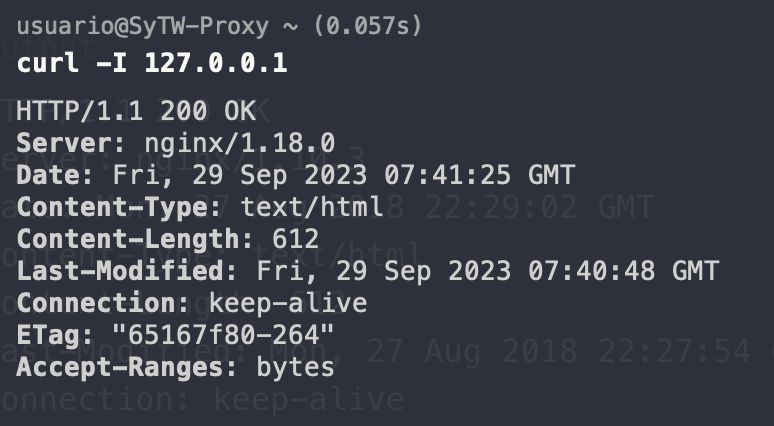
\includegraphics[scale=0.6]{Capturas-Informe-2-STW/Image-1.png}
    \caption{Comprobación del funcionamiento del servidor web Nginx.}
    \label{fig:Comprobación-Nginx}
  \end{figure}

  Para continuar, se realiza la configuración de Nginx en modo \emph{Reverse Proxy}. Para ello, se debe de modificar el fichero de configuración de Nginx que se encuentra en la ruta \emph{/etc/nginx/sites-available/default} y se debe de añadir el siguiente código:

  \begin{verbatim}
    location / {
      proxy_pass http://<IP-MAQUINA-APP>:<PUERTO-APP>;
    }
  \end{verbatim}

  Para este caso, la configuración que se debe de realizar tiene que ser implementada como se puede ver en la figura \ref{fig:Configuración-Reverse-Proxy}.

  \begin{figure}[H]
    \centering
    \includegraphics[scale=0.6]{Capturas-Informe-2-STW/Configuración-Reverse-Proxy.png}
    \caption{Configuración de Nginx en modo Reverse Proxy.}
    \label{fig:Configuración-Reverse-Proxy}
  \end{figure}

  Tras esto, se puede comprobar que el funcionamiento de Nginx ya es correcto. Para ello se acude al navegador y se introduce la siguiente dirección \emph{http://10.6.131.137/}, generando que se muestre el mensaje que se puede ver en la figura \ref{fig:Comprobación-Reverse-Proxy}.

  \begin{figure}[H]
    \centering
    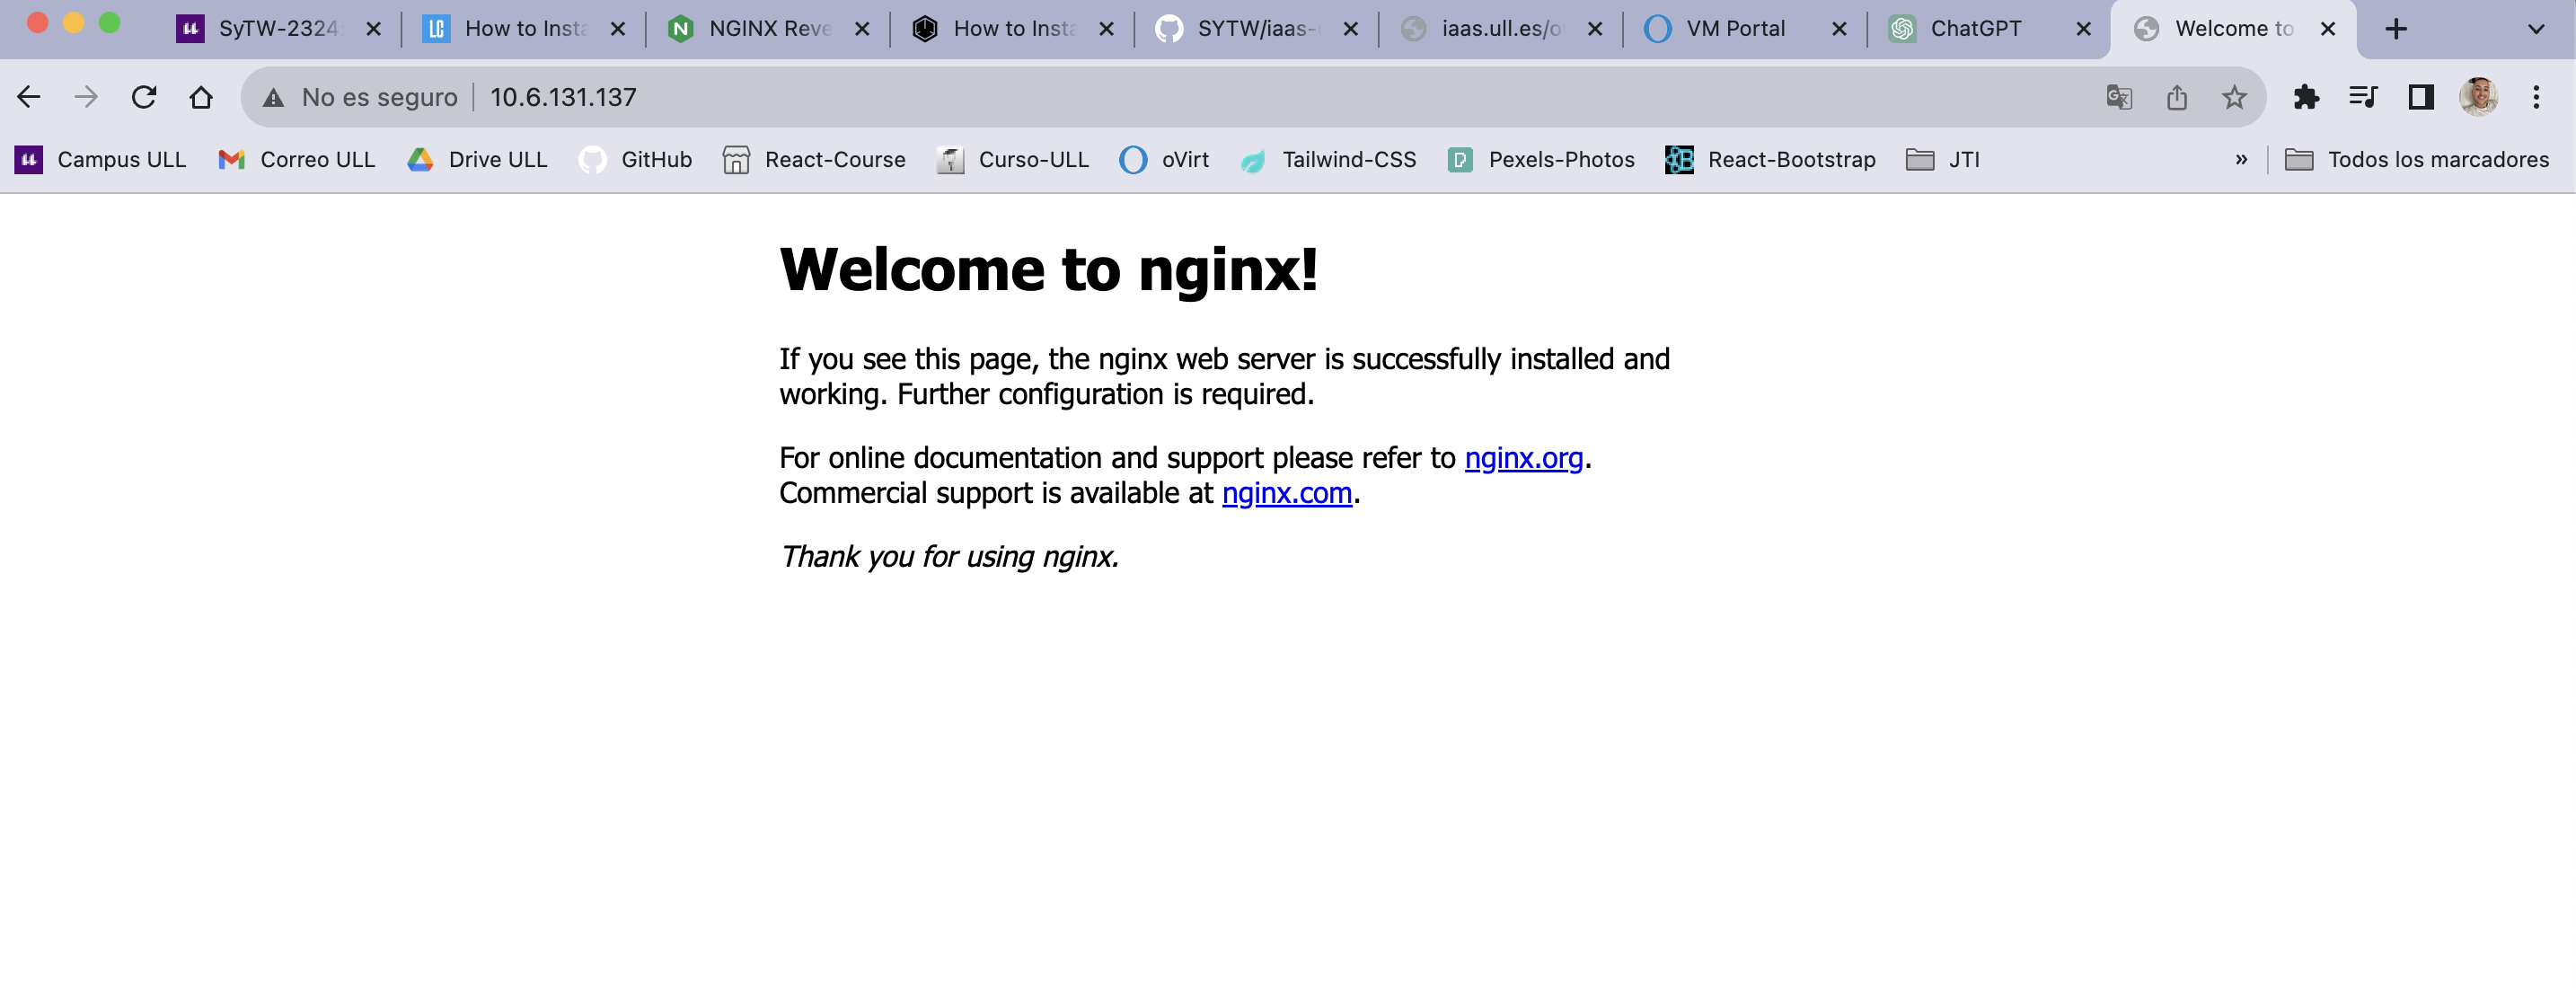
\includegraphics[scale=0.6]{Capturas-Informe-2-STW/Funcionamiento-de-ngingx.png}
    \caption{Comprobación del funcionamiento de Nginx en modo Reverse Proxy.}
    \label{fig:Comprobación-Reverse-Proxy}
  \end{figure}

  Finalmente, tras todos estos pasos, se tiene configurado de manera correcta la máquina virtual Proxy para que funcione como servidor web Nginx en modo Reverse Proxy.

  \chapter{Configuración de la máquina de backend}
  Para esta máquina, se debe de realizar la instalación de \emph{NodeJS}, ya que, será la máquina en la que se desplegara una aplicación de prueba. Es por ello que, para la instalación de NodeJS se hace uso de la siguiente \href{https://linuxconfig.org/how-to-install-nodejs-on-debian-9-stretch-linux}{guía} de instalación.

  Una vez se tiene instalado de manera correcta NodeJS, se puede comprobar su instalación como se puede ver en la figura \ref{fig:Comprobación-NodeJS}

  \begin{figure}[H]
    \centering
    \includegraphics[scale=0.5]{Capturas-Informe-2-STW/Instalación-nodejs.png}
    \caption{Comprobación de la instalación de NodeJS.}
    \label{fig:Comprobación-NodeJS}
  \end{figure}

  Una vez se tiene instalado NodeJS, se procede al despliegue de una pequeña aplicación en \emph{Express} que se encuentra dentro del siguiente \href{https://github.com/crguezl/express-start}{repositorio}. Para ello, se clona dentro de la máquina backend, y, posteriormente se realiza la instalación de todas aquellas dependencias que sean necesarias haciendo uso de \verb|node|: npm install.

  Tras esto, se realiza la configuración de manera correcta del código fuente de la aplicación para que esta se pueda encontrar escuchando el puerto 3000. Es por ello que se modifica el fichero \emph{hello.js} de la manera que se puede observar en la figura \ref{fig:Configuración-puerto-3000}.

  \begin{figure}[H]
    \centering
    \includegraphics[scale=0.6]{Capturas-Informe-2-STW/Modificación-Fichero-HelloJS.png}
    \caption{Modificación del código fuente del fichero Hello.js}
    \label{fig:Configuración-puerto-3000}
  \end{figure}

  Finalmente, se ejecuta la aplicación para que se encuentre en segundo plano escuchando el puerto 3000, para que, posteriormente, cuando el servidor Proxy realice la petición a esta máquina, se pueda obtener una respuesta. Este resultado se puede observar en la figura \ref{fig:Comprobación-Backend}

  \begin{figure}[H]
    \centering
    \includegraphics[scale=0.5]{Capturas-Informe-2-STW/Comprobación-Hello-World.png}
    \caption{Comprobación del funcionamiento del Reverse Proxy.}
    \label{fig:Comprobación-Backend}
  \end{figure}

  \chapter{Configuración de la máquina de bases de datos}
  Para esta máquina, se debe de realizar la instalación de \emph{MongoDB}, es por ello que, se hace uso de la siguiente \href{https://www.mongodb.com/docs/manual/tutorial/install-mongodb-on-debian/}{guía} para su instalación. Pero, de manera previa a la instalación de MongoDB en la máquina implantada en la primera práctica de la asignatura, se debe de realizar la eliminación de esta y la reinstalación de otra nueva que implemente \emph{Debian 12}. Esto, se debe a que la plantilla de \emph{Debian 11} que existe dentro del entorno del IaaS de la ULL, se trata de una máquina de 32 bits la cúal no permite la instalación de MongoDB debido a su antigüedad. Es por ello que, se realiza la instalación de una nueva máquina con \emph{Debian 12} de 64 bits mediante una ISO que se encuentra dentro de dicho entorno del IaaS. Tras esto, se puede observar el resultado final de la instalación en la figura \ref{fig:Comprobación-Debian12}.

  \begin{figure}[H]
    \centering
    \includegraphics[scale=0.4]{Capturas-Informe-2-STW/Instalación-Debian-12.png}
    \caption{Comprobación de la instalación de la máquina virtual de Debian 12.}
    \label{fig:Comprobación-Debian12}
  \end{figure}

  Una vez se tiene instalada la máquina virtual con \emph{Debian 12}, se procede a la instalación de MongoDB haciendo uso de la guía anteriormente mencionada. Tras esto, se realiza la comprobación de la instalación de MongoDB como se puede ver en la figura \ref{fig:Comprobación-MongoDB}.

  \begin{figure}[H]
    \centering
    \includegraphics[scale=0.5]{Capturas-Informe-2-STW/Instalación-MongoDB.png}
    \caption{Comprobación de la instalación de MongoDB.}
    \label{fig:Comprobación-MongoDB}
  \end{figure}

  Para finalizar, se habilita la autenticación en el servidor MongoDB para que se pueda acceder a este mediante un usuario y contraseña, para ello, hacemos uso de la siguiente \href{https://www.mongodb.com/docs/manual/tutorial/enable-authentication/}{guía}. Además, se realiza la creación de un usuario y una base de datos para la aplicación de prueba que se ha desplegado en la máquina de backend de manera previa. Todo esto, queda reflejado en las siguientes figuras \ref{fig:Habilitación-Autenticación-MongoDB} y \ref{fig:Creación-Usuario-App-MogoDB}

  \begin{figure}[H]
    \centering
    \includegraphics[scale=0.6]{Capturas-Informe-2-STW/Creación-Usuario-Admin-MogoDB.png}
    \caption{Habilitación de la autenticación en MongoDB mediante un usuario Admin y contraseña.}
    \label{fig:Habilitación-Autenticación-MongoDB}
  \end{figure}

  \begin{figure}[H]
    \centering
    \includegraphics[scale=0.6]{Capturas-Informe-2-STW/Creación-usuario-para-bdd-test.png}
    \caption{Creación de un usuario y una base de datos para la aplicación de prueba.}
    \label{fig:Creación-Usuario-App-MogoDB}
  \end{figure}

  \chapter{Configuración de la máquina de base de datos para sistema de ficheros compartido}
  Para esta máquina, se debe de realizar la instalación de \emph{NFS} para que se pueda realizar el montaje de un sistema de ficheros compartido entre la máquina de backend y la máquina de bases de datos. Es por ello que, se hace uso de la siguiente \href{https://wiki.debian.org/NFSServerSetup}{guía} para la instalación de NFS.

  \end{document}
